\documentclass[a4paper,11pt]{report}
\usepackage[utf8]{inputenc}
\usepackage{graphicx}
\usepackage{amsmath}
% Title Page
\title{\LARGE{ \textbf{BLG435E}} \\ \vspace{15mm}
Artificial Intelligence\\ \vspace{10mm}  
Assigment 1\\ \vspace{15mm}}

\author{Ozan Arkan CAN\\ 
040090573\\}

\begin{document}
\maketitle

\section*{Question 1}
\emph{\textbf{Home Service Robot}}\\
\\
\textbf{Performance:} Well serving, happiness of owner\\
\textbf{Environment:} Home, People, Stuffs\\
\textbf{Actuators:} Robotic arm\\
\textbf{Sensors:} Motion sensor, optic sensor, infrared sensor etc.\\
\\
\textbf{Partially Observable:} Robot cannot see the whole world.\\
\textbf{Multi Agent:} If people are evaluated as agent than the task has multi agents.\\
\textbf{Stochastic:} There are possible actions that can be done by robot in definete situation. Robot might act different in same situation.\\
\textbf{Sequential:} Actions of robot effect the next situations.\\
\textbf{Dynamic:} Task environment is real world and real world is changing continously.\\
\textbf{Continous:} The actions are executed in continous time.\\
\textbf{Goal based agent:} Aim of the robot is serving to people and its actions are not rule based. Also, robot cannot see the whole world and it might be act depend on its aim. So, robot behaves to achive its goal.\\
\\
\emph{\textbf{A dynamic personalized e-mail organizer for e-mail services}}\\
\\
\textbf{Performance:} High percentage on choosing right category\\
\textbf{Environment:} Web server\\
\textbf{Actuators:} File organizing commands or operating system\\
\textbf{Sensors:} e-mail input\\
\\
\textbf{Fully Observable:} The organizer can see all e-mails.\\
\textbf{Single Agent:} There is only one agent, the organizer.\\
\textbf{Stochastic/Deterministic:} If the organizer is a rule based agent than environment is deterministic, else if organizer decides based on some probabilistic parameters than the environment is stochastic.\\
\textbf{Episodic:} Organizer takes an e-mail and organizes it in one episode. This situation does not effect the next episodes.\\
\textbf{Static:} E-mails are stable.\\
\textbf{Discrete:} Organizer makes an action in periodic time (a few cpu cyles). \\
\textbf{Model based reflex agent:} Organizer might manage the e-mail by rule based or probabilistic model.\\
\\
\emph{\textbf{Autonomous car driver}}\\
\\
\textbf{Performance:} Quicker, Safer, Cheaper\\
\textbf{Environment:} Road, Cars, People\\
\textbf{Actuators:} Wheel, gas pedal, break\\
\textbf{Sensors:} Optic sensor, infrared sensor etc.\\
\\
\textbf{Partially Observable:} Driver can see only its near circle.\\
\textbf{Multi Agent:} There are another cars.\\
\textbf{Stochastic:} There are many options in any situation and driver can chose one of them.\\
\textbf{Sequential:} Actions of driver are done by an order.\\
\textbf{Dynamic:} Task environment is real world and real world is changing continously.\\
\textbf{Continous:} The actions are executed in continous time. \\
\textbf{Utility based agent:} There are many goals such as time, money, safety. Driver can act according these goals to maximize the outcome.\\
\\
\emph{\textbf{Activity recognition and anomaly detection software agent}}\\
\\
Assumption: The task is observing air traffic and detecting anomaly.\\
\\
\textbf{Performance:} Detecting any anomaly\\
\textbf{Environment:} Radar system\\
\textbf{Actuators:} communication system\\
\textbf{Sensors:} Radars, flight data\\
\\
\textbf{Fully Observable:} Data of every flights can be reachable digitally.\\
\textbf{Single Agent:} Planes are object in this task.\\
\textbf{Stochastic/Deterministic:} Agent might have model to act but if its rule based than the environment is deterministic else the environment is stochastic.\\
\textbf{Sequential:} Task is holding in an order like observe, detect, act.\\
\textbf{Dynamic:} Task is detecting anomaly, so environment must be changeble.\\
\textbf{Continous:} The actions are executed in continous time. \\
\textbf{Model based reflexagent:} Agent needs model to detect anomaly. It could be probabilistic or rule based.\\
\\
\newpage 

\section*{Question 2}

If algorithm is consistent, for every node n and every successor n' of n generated by any action a, than the estimated cost of
reaching the goal from n less or equals than the step cost getting to n' plus the estimated cost of reaching the goal
from n'.\\
\\
$ h(n) < c(n,a,n') + h(n') $ (Triangle Inequality)\\
\begin{math}
 f(n') = g(n') + h(n')\\
 f(n') = g(n) + c(n,a,n') + h(n')\\
 f(n') \geq g(n) + h(n)\\
 f(n') \geq f(n)\\
\end{math}
\\$f(n)$ is nondecreasing on any path.\\
\\
Let n is start node, n' is the successor and g is the goal node.\\
Assume that:\\
\\$c(n,a,n') = 1$ , $c(n,a,g) = 10$ , $c(n',a,g) = 10$\\ (Actual costs with Triangle Inequality, Admissible) and\\
\\$h(n) = 8$ , $h(n') = 6$\\
$h(n) > h(n') + c(n,a,n')$ Inconsistency\\
\newpage

\section*{Question 3}
\subsection*{Problem Definition}
\textbf{Initial State: }Given board configuration is initial state.\\
\textbf{Actions: }Vertical blocks can move along y axis, horizontal blocks can move along x axis.
They are moved while there is no another block or it is not near the border.\\
\textbf{Transition Model: }After an action has done, the result is new board configuration.\\
\textbf{Goal Test: }The goal is moving the target block to gate which is at 3rd row, 6th column. 
Goal test is controlling the whether the target block is at gate or not.\\
\textbf{Path Cost: }Path cost is number of moves for sliding a block in each action.\\ 
\subsection*{Analysis of Uninformed Search Algorithm}
In this chapter, the worst case senario is given belove for the analysis:\\
-All cells that are on the path which is between target block and gate are occupied. This means there are 4 blocks.\\
-There are anothor blocks on those blocks. This adds 4 blocks more.\\
\\So, 8 blocks must be moved to target block can move.\\
According this information number of branch is number of total blocks. The maximum depth of tree is $m = 8 + 1 = 9$ 
(The one comes for moving the target block to gate.)

\subsubsection*{Breadth First Search}
The BFS algorithm searches the tree layer by layer. In this problem this facility means in each action a block 
that has not been moved in layer is moved. This cause if node that is on the first places belongs to solution path, 
searching the remained nodes in the layer slowdowns the algoritm, but algorithm is available for finding optimal solution.
Because the path costes are nondecreasing.\\
So, time complexity is $O(b^{d})$, space complexity is $O(b^{d})$.

\subsubsection*{Depth First Search}
The DFS searches the tree following branches step by step. According the problem this algorithm can be stack a branch because, 
algorithm can move a block right to left, left to right or top to down, down to top forever. But if we create a definite search space(give a tree the algorithm in order to creating running time)
the algorithm can reach the solution. The running time of algorithm is $O(b^{m})$ and the space complexity is $O(bm)$.

\subsubsection*{Uniform-cost Search}
The Uninform-cost search algorithm has same strategy with BFS algorithm, but there is a difference to struct the queue. 
The algorithm expands the nodes by their path cost as ascending order. So, algorithm chooses node that has smallest path cost in that layer. 
By this strategy, algorithm reaches the solution faster than BFS.\\ The running time and the space complexity are same as complexities of BFS, but this analysis is for worst case. 
In average case, complexties decrease by path cost.

\subsection*{Implementation of A* Algorithm}
\subsubsection*{Algorithm Definition}
In this program, A* algorithm is implemented to solve the program. It is a kind of best-search algorithm.
Node selection depends on the total cost. A heuristic algorithm like A* needs two function 
which are cost for reaching current node and the cost of heuristic value for reaching the goal node.
In this program, two different heuristic functions are used to calculate the heuristic cost.\\
\textbf{Heuristic Function1:} Number of moves for moving target block to gate.\\
\textbf{Heuristic Function2:} Number of blocks on the path that is from target block to gate.\\
\textbf{Path Cost ($g(n)$):} Path cost is number of moves for sliding a block in that node.\\
\\textbf{Total Cost: } $f(n) = g(n) + h(n)$\\
\\
In this implementation a priority queueu is used as frontier and the nodes are sorted depends on their total cost in 
ascending order.

\subsubsection*{Development Environment}
The program has been develop with \textit{Eclipse} development environment on Fedora17 64 bit system. 
It has been build and run from this ide. Program can be run with non parameters or with 3 tree parameters which are 
path for input file, path for outputfile and number of herustic function that is used to calculate cost.\\
There is also a folder that contains all java files with a makefile. Files can be build and run without ide.\\
\\
\textbf{To build:} make\\
\textbf{To run:} java Mainprogram or java Mainprogram inputFilePath outputFilePath choiceForHeuristicFunction\\
\textbf{To clean:} make clean\\

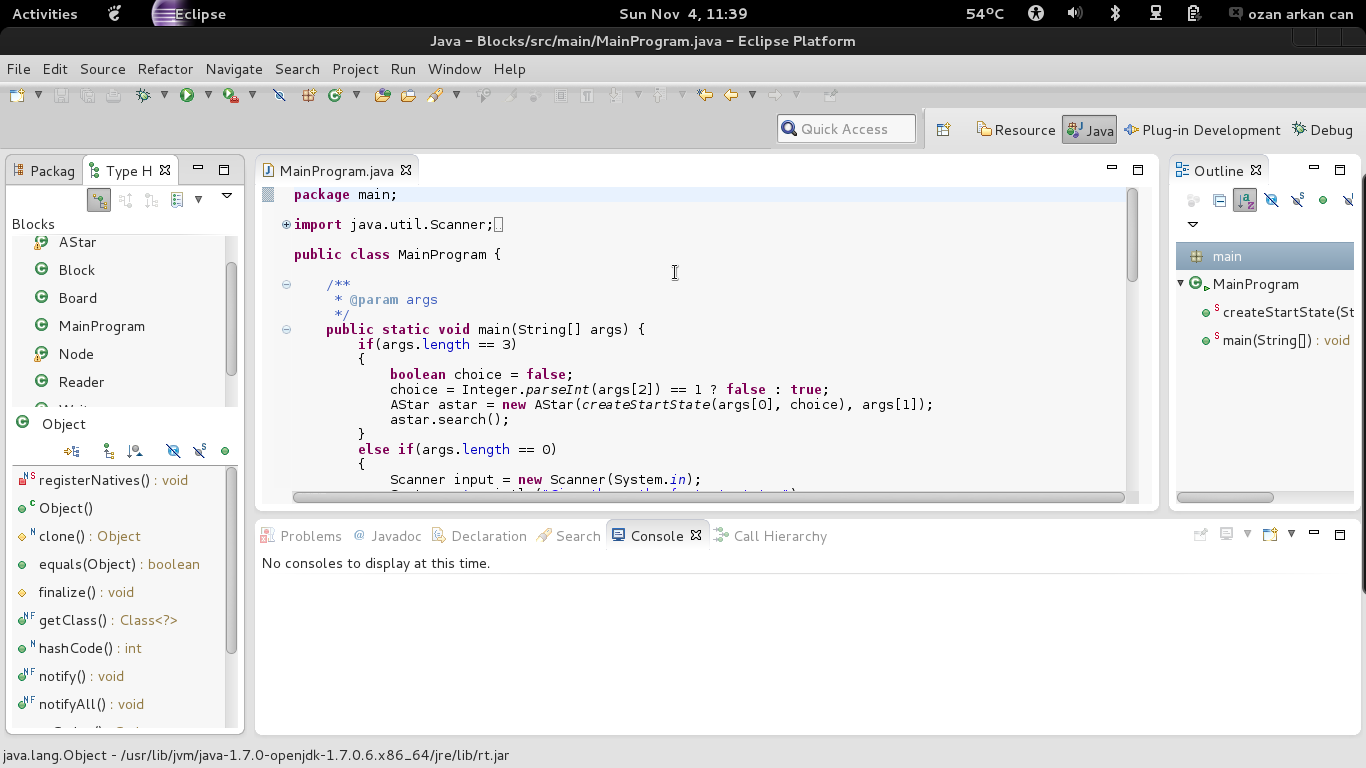
\includegraphics[scale=0.3]{develop}
\newpage
\subsubsection*{UML Diagram}

The UML diagram of the program is given belove.\\

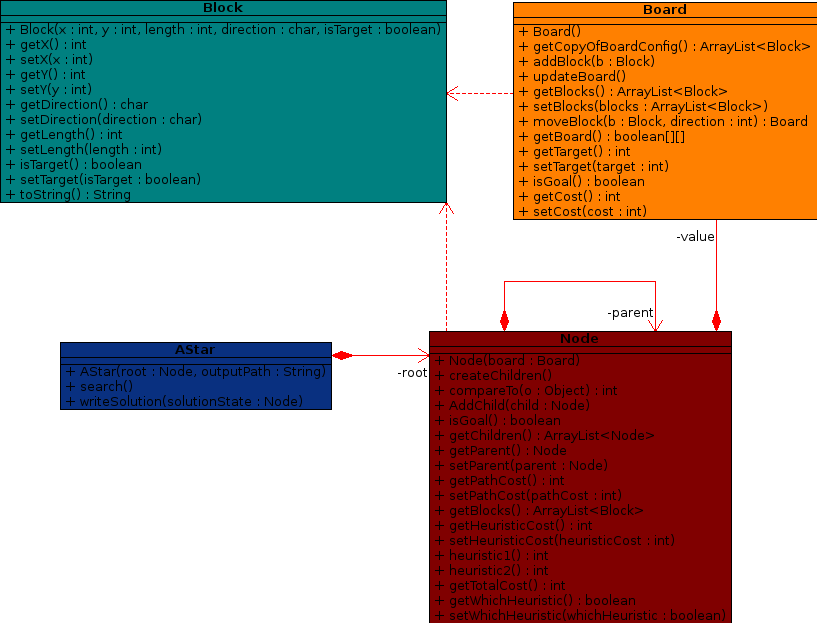
\includegraphics[scale=0.6]{blocksUml}

\subsubsection*{Algorithm Analysis}

Implemented A* algorithm run with two different heuristic functions. Strategy for the first function is choosing 
the node that has nearest target block to gate. But this function misses the number of moves that for cleaning the path. 
So there are a lot of nodes that has same heuristic value and decision for choosing the node effects the algorithm complexity.\\
Second heuristic function aims to remove the blocks that are between target block and gate. Algorithm slides a block if the block on the path 
or the block must be moved for removing the obstacle block. Algorithm cannot visit any node again because the costs are nondecreasing. 
In conclusion, A* algorithm is faster than uninformed algortihms and second heuristic function works better than other.\\

\section*{Conclusion}

This assigment helps to exercise the following issues:\\

\begin{itemize}
 \item To define a problem
 \item To define properties of environment and PEAS components
 \item To define an agent
 \item Uninformed and heuristic algorithms
 \item Data Structures
\end{itemize}

\end{document}          
